\documentclass{extreport}

\usepackage[14pt]{extsizes}
\usepackage[T2A]{fontenc}
\usepackage[utf8]{inputenc}
\usepackage[english,ukrainian]{babel}

\usepackage[a4paper, top=10mm, bottom=15mm, left=20mm, right=15mm]{geometry}
\usepackage{amsmath,amsfonts,amssymb,amsthm,mathtools}
\usepackage{listings}
\usepackage{graphicx}
\usepackage{enumitem}
\usepackage{verbatim}
\usepackage{listings}
\usepackage{xcolor}
\usepackage{textgreek}
\usepackage{diagbox}
\usepackage{pgfplots}
\pgfplotsset{compat = 1.16}


\lstdefinestyle{output_txt}{
    basicstyle=\ttfamily\footnotesize,
    breakatwhitespace=false,         
    breaklines=true,                 
    captionpos=b,                    
    keepspaces=true,                                    
    numbersep=5pt,                  
    showspaces=false,                
    showstringspaces=false,
    showtabs=false,                  
    tabsize=2
}
\definecolor{codegreen}{rgb}{0,0.6,0}
\definecolor{codegray}{rgb}{0.5,0.5,0.5}
\definecolor{codepurple}{rgb}{0.58,0,0.82}
\lstdefinestyle{python_code}{ 
    commentstyle=\color{codegreen},
    keywordstyle=\color{magenta},
    numberstyle=\tiny\color{codegray},
    stringstyle=\color{codepurple},
    basicstyle=\ttfamily\footnotesize,
    breakatwhitespace=false,         
    breaklines=true,                 
    captionpos=b,                    
    keepspaces=true,                            
    numbersep=5pt,                  
    showspaces=false,                
    showstringspaces=false,
    showtabs=false,                  
    tabsize=4
}

\setlist[enumerate]{nosep}
\graphicspath{{pics/}}
\DeclareGraphicsExtensions{.png}

\begin{document}
\begin{titlepage}
    \thispagestyle{empty}
    \begin{center}
        
\includegraphics[width = \textwidth]{kpi}
        Міністерство освіти і науки України\\
        Національний технічний університет України\\
        <<Київський політехнічний інститут ім. І. Сікорського>>\\
        Інститут прикладного системного аналізу
    \end{center}
    \vspace{40mm}
    \begin{center}
        \textbf{Лабораторна робота} \\
        з курсу <<Методи оптимізації>> \\
        з теми <<Чисельні методи безумовної оптимізації другого порядку. 
        Метод Ньютона та його варіації>>
    \end{center}
    \vspace{20mm}
    \begin{flushleft}
        Виконали студенти 3 курсу групи КА-81 \\
        Галганов Олексій \\
        Єрко Андрій \\
        Фордуй Нікіта
    \end{flushleft}
    \begin{flushright}
        Перевірили \\
        Спекторський Ігор Якович \\
        Яковлева Алла Петрівна
    \end{flushright}
    \vspace{30mm}
    \begin{center}
        \textbf{Київ 2021}
    \end{center}
\end{titlepage}

\begin{center}
    \textbf{Варіант 1}
\end{center}
\textbf{Завдання.} Скласти програму для мінімізації цільової функції
одним з методів другого порядку (типу Ньютона). Конкретний тип методу обрати
самостійно, ураховуючи особливості цільової функції.

\emph{Цільова функція:}
$f(x,y) = x^2 + 18y^2 + 0.01xy + x - y$

\noindent\textbf{Результати роботи.}
Цільова функція є квадратичною, а тому використовувати узагальнені методи немає сенсу,
оскільки класичний метод Ньютона: $x^{k+1} = x^k - [f''(x^k)]^{-1} f'(x^k)$
для квадратичний функцій знаходить розв'язок за одну ітерацію.

Доведемо для $\mathbb{R}^2$: \\
Розглядаємо строго опуклі $f$ виду
$$f(x,y) = Ax^2 + By^2 + Cxy + Dx + Ey + F, $$
Тоді: $$f'(x,y) = \begin{pmatrix}
    2Ax + Cy + D \\
    Cx + 2By + E
\end{pmatrix}$$
$$ f''(x,y) = H  = \begin{pmatrix}
    2A & C \\
    C & 2B
\end{pmatrix}$$

Тоді будь-яке початкове наближення $\vec x_0$ представимо у вигляді
$\vec x_0 = \vec x^* + \vec r$, де $\vec x^*$ - шуканий розв'язок (єдиний з умови строгої опуклості)
$$\vec h = H^{-1} f'(\vec x_0)$$
$$H \vec h = f'(\vec x^* + \vec r)$$
$$ \begin{pmatrix}
    2Ah_1 + Ch_2 \\
    Ch_1 + 2Bh_2
\end{pmatrix} =
\begin{pmatrix}
    \overbrace{2Ax^* + Cy^* + D}^{0} + 2Ar_1 + Cr_2\\
    \underbrace{Cx^* + 2By^* + E}_{0} + Cr_1 + 2Br_2
\end{pmatrix}$$
$$ \begin{pmatrix}
    2Ah_1 + Ch_2 \\
    Ch_1 + 2Bh_2
\end{pmatrix} =
\begin{pmatrix}
    2Ar_1 + Cr_2\\
    Cr_1 + 2Br_2
\end{pmatrix}$$
Звідки отримуємо рівність $\vec h = \vec r$. $\qed$ 

Оскільки обраний критерій зупинки --- $\left| f(x_{k+1}) - f(x_k)\right| < \varepsilon = 10^{-5}$
вимагає принаймні дві ітерації для порівняння, було отримано збіжність до точки мінімуму за 2 ітерації.
\begin{center}
    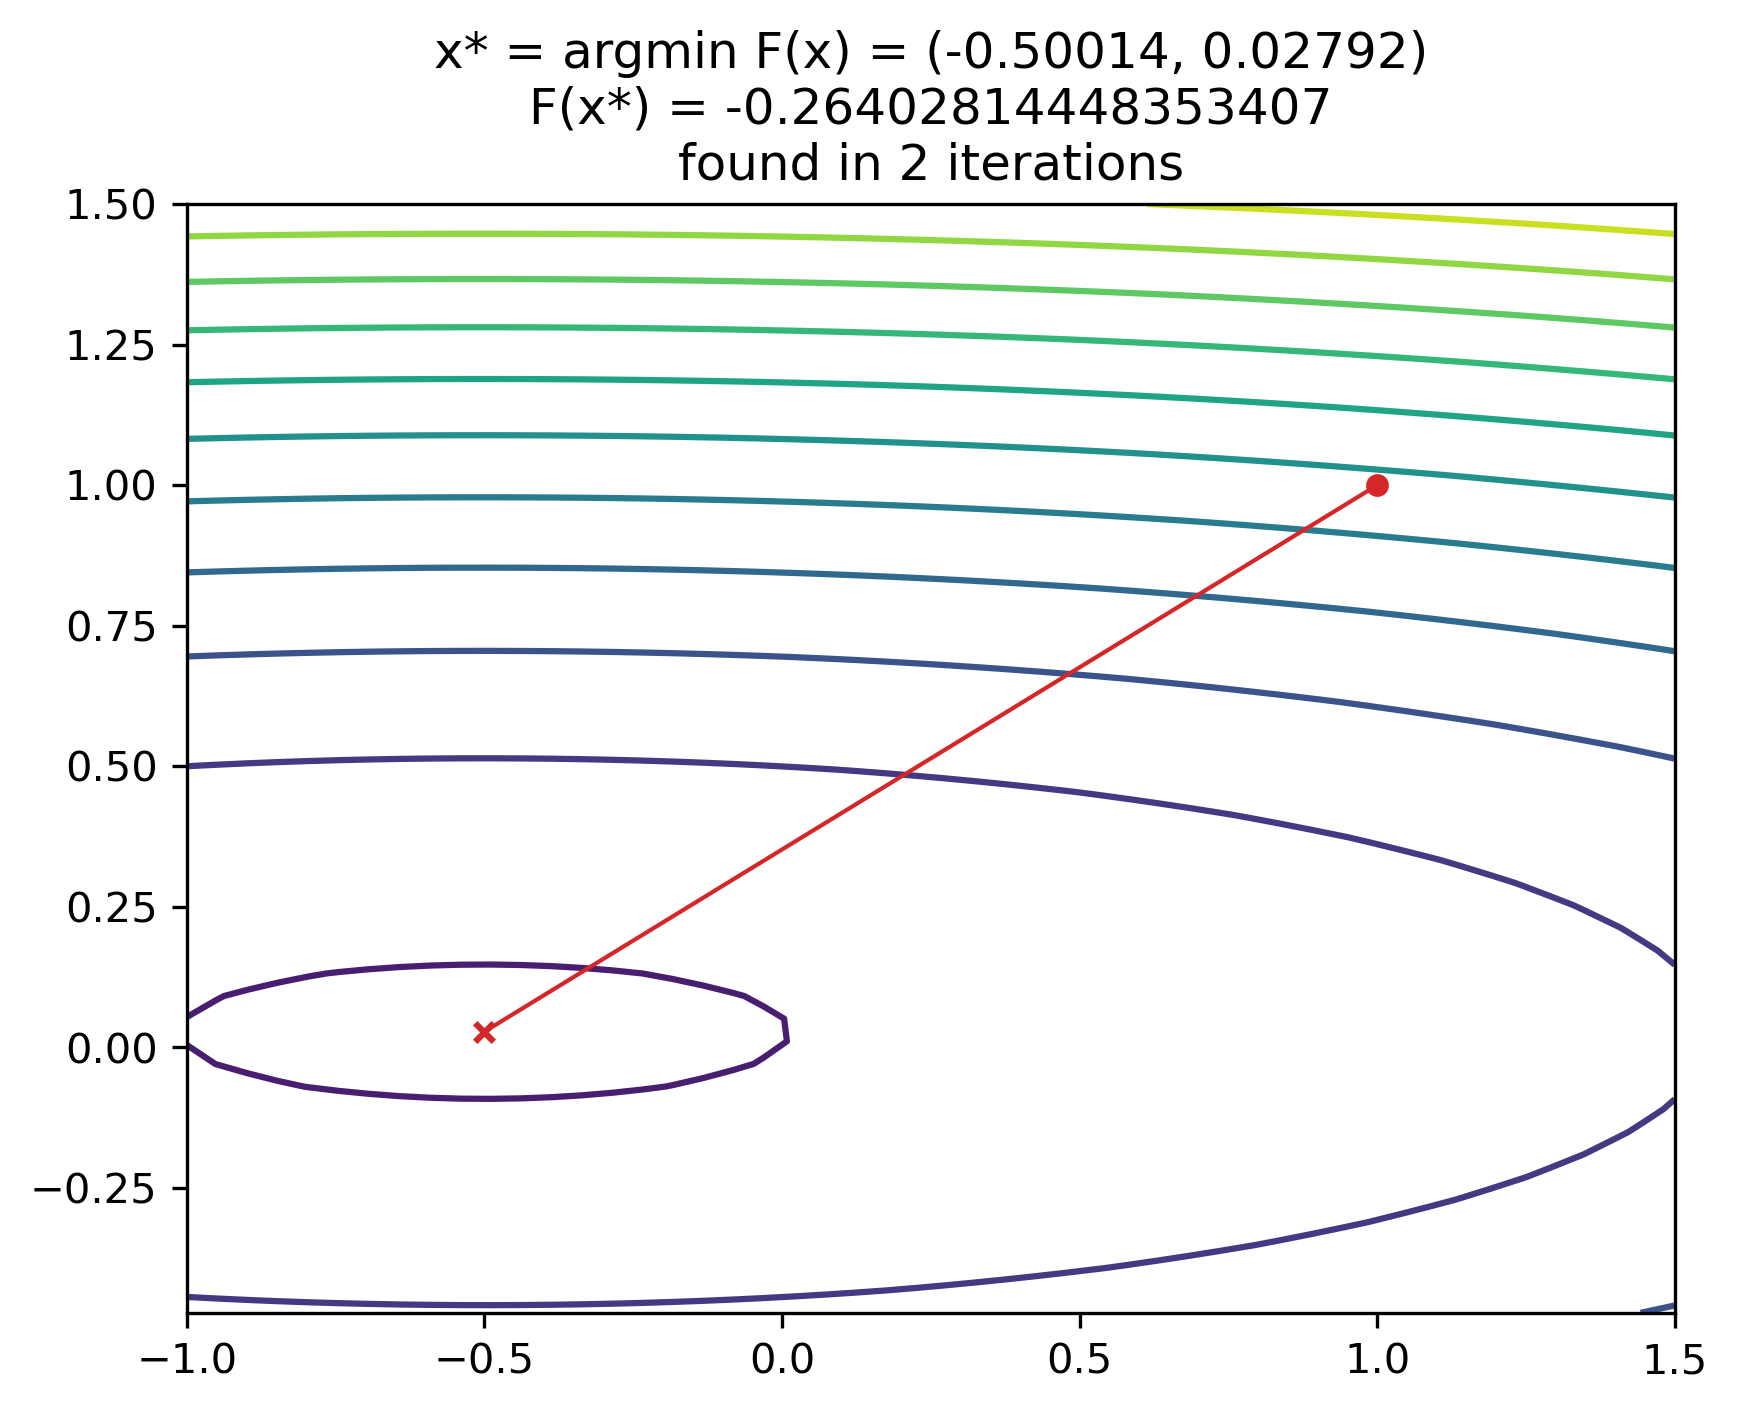
\includegraphics[scale = 0.8]{contour_final.png}
\end{center}

\noindent\textbf{Лістинг.}
Текст програми було розділено на \texttt{Optimizer.py} з реалізацією
власне методу Ньютона та \texttt{lab2.py}, де він викликається та зберігаються результати.

\noindent\texttt{Optimizer.py}
\lstinputlisting[language = Python, style = python_code]{../code/Optimizer.py}

\noindent\texttt{lab1.py}
\lstinputlisting[language = Python, style = python_code]{../code/lab2.py}

\noindent\textbf{Висновки.} При виконанні даної роботи ми дослідили
застосування методу Ньютона до мінімізації заданої функції.
Оскільки мінімум квадратичної функції може бути знайдений класичним методом Ньютона
за одну ітерацію, було реалізовано саме його, а відповідний факт доведено для функцій двох змінних.
\end{document}